\author{Gottfried von Recum}

\section{Browser}

Denkbare Use Cases des Browsers sind:
\begin{figure}[h]
	\centering
	\includegraphics[width=0.6\textwidth]{use_case_browser1}
	\caption{Use Case des Browsers}
	\label{fig:Browser Use-Case}
\end{figure}
\begin{figure}[h]
	\centering
	\includegraphics[width=0.6\textwidth]{use_case_browser2}
	\caption{Use Case des Browsers}
	\label{fig:Browser Use-Case}
\end{figure}
\begin{figure}[h]
	\centering
	\includegraphics[width=0.6\textwidth]{use_case_browser3}
	\caption{Use Case des Browsers}
	\label{fig:Browser Use-Case}
\end{figure}
\pagebreak

\begin{figure}[h]
	\centering
	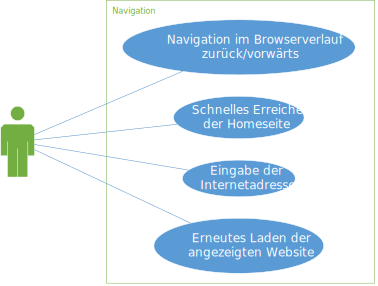
\includegraphics[width=0.6\textwidth]{USECASE_Nutzer_Browser_Navigation}
	\caption{Use Case der Browser Navigation}
	\label{fig:Browser Navigation Use-Case}
\end{figure}
\pagebreak

\begin{figure}[h]
	\centering
	\includegraphics[width=0.6\textwidth]{USECASE_Nutzer_Lesezeichen}
	\caption{Use Case der Browser Lesezeichen}
	\label{fig:Browser Lesezeichen Use-Case}
\end{figure}
\pagebreak

\begin{figure}[h]
	\centering
	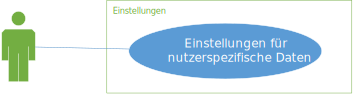
\includegraphics[width=0.6\textwidth]{USECASE_Nutzer_Einstellungen}
	\caption{Use Case der Browser Einstellungen}
	\label{fig:Browser Einstellungen Use-Case}
\end{figure}
\pagebreak